\begin{savequote}[45mm]
\ascii{Any fool can write code that a computer can understand. Good programmers write code that humans can understand.}
\qauthor{\ascii{- Martin Flower}}
\end{savequote}

\chapter{xUnit架构} 
\label{ch:xunit-architecture}

\begin{content}

本章重点介绍\ascii{xUnit}的基本框架与测试方法论,通过讨论\ascii{Google Test}框架的优缺点,引入\ascii{xUnit Mars}框架,重起炉灶,再造轮子。最后,简单介绍\ascii{xUnit Mars}的用例风格与系统架构。

通过\ascii{xUnit Mars}的设计与实现,探究\ascii{TDD},重构与简单设计的实践过程,并深入体会正交设计、设计原则、设计模式、整洁代码、实现模式与习惯用法在编程实践中的具体运用。

% 本书通过使用\cpp{}设计和实现\ascii{xUnit}框架,透视极限编程在\cpp{}社区中的具体实践与运用,包括\ascii{简单设计},\ascii{TDD}、重构。

% 也会深入体会正交设计、设计原则、设计模式、整洁代码、实现模式与习惯用法在编程实践中的具体运用;也会在面向对象、函数式、泛型编程不同编程范式之间切换自如;也会尝试\ascii{DSL}设计与实现,体会代码之美,设计之美,架构之美。

\end{content}

\section{xUnit族谱}

\begin{content}

\subsection{开山鼻祖}

\ascii{xUnit}表示一组单元测试框架集合,其基本思想起源于\ascii{SUnit}。\ascii{SUnit}由极限编程之父\ascii{Kent Beck}使用\ascii{SmallTalk}设计实现。随后,\ascii{Kent Beck}与\ascii{Erich Gamma}结对编程,移植实现了\ascii{Java}版本\ascii{JUnit}。

\ascii{JUnit}随着\ascii{Java}社区不断壮大,及其敏捷软件开发思潮的涌现,当前\ascii{JUnit}已经成为\ascii{Java}程序员最常使用的框架之一。而且\ascii{JUnit}也在不断地进化与演进,截止目前\ascii{JUnit5}已然面世,重焕青春。

随之各家语言社区都诞生了自家优秀的\ascii{xUnit}实现,包括基于\ascii{JVM}实现的各种高级编程语言。但是,它们都基本继承或发扬了\ascii{xUnit}基本架构与方法论,部分后起之秀在用户界面友好性方面也取得极大的改进和提升。例如,我所偏爱的\ascii{Spock, ScalaTest}框架。

\subsection{名家之作}

\ascii{Google Test}出自\ascii{Google},自带光环。其使用\cpp{}语言实现,其功能强大,系统稳定,移植性良好,支持用例自动发现,相对于\cpp{}社区其它\ascii{xUnit}实现更显技高一筹,在\cpp{}社区占据主导地位。

\begin{nodiff}{Google Test样例}
 \begin{c++}
#include <gtest/gtest.h>
#include <stack>

namespace {
  struct StackSpec : testing::Test {
  private:
    void SetUp() override {
      s.push(1);
      s.push(2);
    }

  protected:
    std::stack<int> s;
  };
}

TEST_F(StackSpec, apply_pop_0_time) {
  ASSERT_EQ(2, s.top());
}

TEST_F(StackSpec, apply_pop_1_time) {
  s.pop();
  ASSERT_EQ(1, s.top());
}

TEST_F(StackSpec, apply_pop_2_time) {
  s.pop();
  s.pop();
  ASSERT_TRUE(s.empty());
}
 \end{c++}
\end{nodiff}

但是,\ascii{Google Test}也存在一些不尽人意的细节之处。

\subsubsection{命名}

用例名字必须遵循标识符的严格命名格则,否则编译不能通过。一方面,新增/修改用例时,输入长串下划线极度枯燥乏味;另一方面,极大地降低了用例的可读性。

当用例命名成为程序员的一种负担,其质量将大大折扣。但是,测试用例是系统行为描述最重要的活“文档”,它与被测系统的代码一并入库,并保持同步。如果,测试用例命名质量不高,\ascii{"Test as Document"}的愿景只能沦为痴人说梦了。

\begin{nodiff}{坏味道:使用标识符命名用例}
 \begin{c++}
// Bad Smell: test cases must be named using c++ identifier.
TEST_F(RobotCleanerTest, at_beginning_the_robot_should_be_in_at_the_initial_position) {
  ASSERT_EQ(Position(0, 0, NORTH), robot.getPosition());
}
 \end{c++}
\end{nodiff}

\subsubsection{重复}

\ascii{RobotCleanerTest}扮演\emph{测试装置},但与每个测试用例(\ascii{TEST\_F})分离实现,每个用例不得不一次次地重复\ascii{RobotCleanerTest}。

测试装置与测试用例相分离,破坏了它们之间的内聚性。当然,\ascii{C++}程序员已然习惯类定义与成员函数定义相分离的思维模式,习惯性接受这样的重复设计。但是,这两种场景存在微妙的差异。

一般地,在\cpp{}编译模型中,头文件中定义类,实现文件中定义成员函数。但是,此处测试装置与测试用例已经在同一个文件内,分离定义而导致重复引入\ascii{RobotCleanerTest},显然给用户增加无畏的负担。

\begin{nodiff}{重复设计:测试装置与测试用例相分离}
 \begin{c++}
struct RobotCleanerTest : testing::Test {
protected:
  RobotCleaner robot;
};
 
// Bad Smell: you must duplicate fixture name for each test case.
TEST_F(RobotCleanerTest, at_beginning_the_robot_should_be_in_at_the_initial_position) {
  ASSERT_EQ(Position(0, 0, NORTH), robot.getPosition());
}
 
TEST_F(RobotCleanerTest, robot_should_be_face_west_after_turn_left) {
  robot.turnLeft();
  ASSERT_EQ(Position(0, 0, WEST), robot.getPosition());
}
  \end{c++}
\end{nodiff}

\subsubsection{隐晦}

测试装置与测试用例相分离,本应该被直观地理解为类与成员函数之间的关系。也就是说,\ascii{TEST\_F}理论上能够直接获取到私有成员\ascii{RobotCleanerTest::robot}。

不幸的是,\ascii{RobotCleanerTest}与\ascii{TEST\_F}存在隐晦的继承关系。如果用户不了解\ascii{Google Test}的实现机制,就根本无法理解成员变量\ascii{RobotCleanerTest::robot}为什么是\ascii{protected},而不是\ascii{private}。

\begin{nodiff}{错误:本应该使用protected,而错误地使用private}
 \begin{c++}
struct RobotCleanerTest : testing::Test {
private: // Error: should be protected
  RobotCleaner robot;
};
 
TEST_F(RobotCleanerTest, at_beginning_the_robot_should_be_in_at_the_initial_position) {
  ASSERT_EQ(Position(0, 0, NORTH), robot.getPosition());
}
  \end{c++}
\end{nodiff}

\subsubsection{误用}

用户也需要关注\ascii{TEST, TEST\_F}之间的区别,及其使用场景,无疑增加了用户的心智包袱。例如,用户在此处本应使用\ascii{TEST\_F},而误用为\ascii{TEST}。这个例子较为幸运,编译器提示\ascii{robot}变量未定义。但是,在特殊场景可能会逃出编译时检查,导致运行时用例失败。

\begin{nodiff}{错误:本应该使用TEST\_F,而错误地使用TEST}
 \begin{c++}
struct RobotCleanerTest : testing::Test {
protected:
  RobotCleaner robot;
};

// Error: should be TEST\_F
TEST(RobotCleanerTest, at_beginning_the_robot_should_be_in_at_the_initial_position) {
  ASSERT_EQ(Position(0, 0, NORTH), robot.getPosition());
}
  \end{c++}
\end{nodiff}

\subsubsection{大小写}

覆写\ascii{Test::SetUp}时,经常将其错误地写为\ascii{setup, setUp, Setup},不经意地大小写错误可能导致运行时测试用例执行失败。当然,如果坚持使用\ascii{override}关键字,可以提高编译时安全性,将错误拦截至编译期。

\begin{nodiff}{错误:本应该声明为SetUp,而错误地声明为Setup}
 \begin{c++}
struct RobotCleanerTest : testing::Test {
private:
  // Error: should override SetUp, not Setup/setup/setUp.
  void Setup() {
    robot.reset();
  }
 
protected:
  RobotCleaner robot;
};
  \end{c++}
\end{nodiff}

\subsection{拙作}

假定预开发的系统名为\ascii{xUnit Mars},它完成类似\ascii{Google Test}的功能特性。相对于\ascii{Google Test},\ascii{xUnit Mars}定义了一套更人性化的\ascii{DSL},改善了用例描述的表达力。

\begin{enum}
  \eitem{使用字符串描述用例,改善用例的表达力;}
  \eitem{在同一个类域内,使得测试用例与测试装置之间的关系更加内聚;}
  \eitem{避免\code{setup/setUp/SetUp}大小写混用而引发错误。}
\end{enum}

\begin{nodiff}{xUnit Mars样例}
 \begin{c++}
#include <mars/mars.h>
#include <stack>

FIXTURE(StackSpec) {
  std::stack<int> v;   

  SETUP {
    v.push(1);
    v.push(2);
  }

  TEST("apply pop: 0 time") {
    ASSERT_EQ(2, v.top());
  }

  TEST("apply pop: 1 time") {
    v.pop();
    ASSERT_EQ(1, v.top());
  }

  TEST("apply pop: 2 times") {
    v.pop();
    v.pop();
    ASSERT_TRUE(v.empty());
  }
}; 
 \end{c++}
\end{nodiff}

\end{content}

\section{系统架构}
	
\begin{content}

\ascii{xUnit Mars}功能特性与\ascii{Google Test}存在明显的重合度。但是,\ascii{xUnit Mars}的用例设计风格与系统架构,相比\ascii{Google Test}存在巨大的差异。

在开发初期,\ascii{xUnit Mars}使用\ascii{Google Test}作为\ascii{TDD}的开发工具,待\ascii{xUnit Mars}完成基本功能,并发布稳定版本之后,可将既有测试用例重构为\ascii{xUnit Mars}风格。基于\ascii{xUnit Mars}基本特性,可以改善使用\ascii{Modern C++}开发各类应用程序的用户体验。初步预想,\ascii{xUnit Mars}系统架构如\refig{mars-framework}所示。

\begin{figure}[H]
\centering
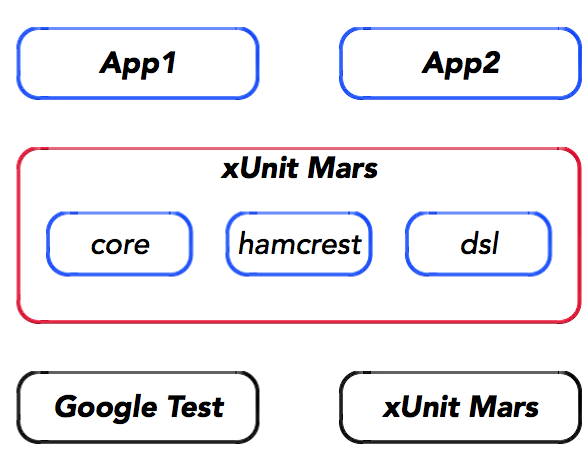
\includegraphics[width=0.5\textwidth]{figures/xunit/framework.png}
\caption{xUnit Mars: 系统架构}
 \label{fig:mars-framework}
\end{figure}

\begin{episode}{代码风格}
\begin{content}

\emph{团队成员遵循\ascii{XP}基本价值观,致力于优秀的软件设计。}系统中所有的代码看起来就好像是由单独一个值得胜任的人编写的,并遵循一致的、统一的的代码风格。

可以配置\ascii{Eclipse CDT}代码模板,团队通过导入代码模板,使其得到一致的代码风格。业界存在多种经典的代码风格,团队应该选择并保持其中一种代码风格。

\begin{enum}
  \eitem{\code{K\&R}}
  \eitem{\code{BSD/Allman}}
  \eitem{\code{GNU}}
  \eitem{\code{Whitesmiths}}
\end{enum}

本书使用\ascii{K\&R}的代码风格,但在对齐方面做了细微调整,如\refig{eclipse-formatter}所示。配置完毕之后,便可以充分享受神奇带来的快感。

\begin{figure}[H]
\centering
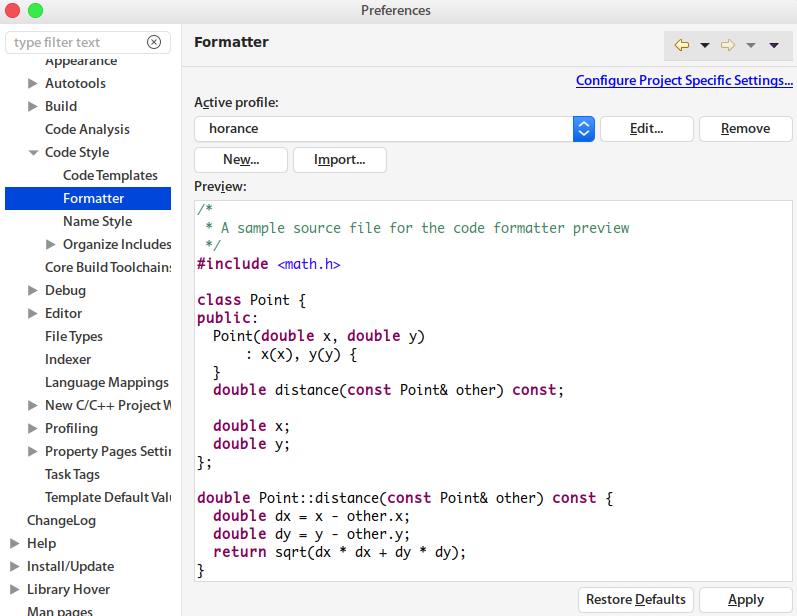
\includegraphics[width=1.0\textwidth]{figures/xunit/eclipse-formatter.png}
\caption{代码风格: K\&R}
 \label{fig:eclipse-formatter}
\end{figure}

例如,创建头文件时,自动生成\ascii{UUID}的头文件保护宏,彻底抛弃这个遗留问题;当需要排版代码时,使用快捷键\ascii{Ctrl + Shift + F}立马得到漂亮的代码风格。

关于\ascii{Eclipse CDT}详细配置与使用技巧,推荐阅读王博\footnote{\href{https://www.jianshu.com/u/92b7d9879f20}{\ascii{https://www.jianshu.com/u/92b7d9879f20}}}在简书上的三篇博文:\href{https://www.jianshu.com/p/dafcdce1f9cb}{\ascii{Effective Eclipse CDT}}。

\end{content}
\end{episode}

\end{content}
